\documentclass[11pt,a4paper]{article}

% --- Språk & typografi ---
\usepackage[T1]{fontenc}
\usepackage[utf8]{inputenc}
\usepackage[swedish]{babel}
\usepackage{lmodern}
\usepackage{microtype}
\usepackage{tikz}

% --- Layout ---
\usepackage{geometry}
\geometry{margin=22mm}
\setlength{\parindent}{0pt}
\setlength{\parskip}{6pt}

% --- Rubriker & sidhuvud ---
\usepackage{titlesec}
\usepackage{fancyhdr}
\pagestyle{fancy}
\fancyhf{}
\lhead{MVE655 — Teorilista (övningsmall)}
\rhead{\thepage}
\renewcommand{\headrulewidth}{0.4pt}

% --- Länkar (valfritt, men bra för TOC) ---
\usepackage[hidelinks]{hyperref}

% --- Boxar för svar ---
\usepackage{xcolor}
\usepackage[most]{tcolorbox}
\tcbset{
  colback=gray!3,
  colframe=gray!35,
  boxrule=0.6pt,
  arc=2mm,
  left=2.5mm,right=2.5mm,top=2mm,bottom=2mm,
  breakable
}

\newtcolorbox{AnswerBox}[2][]{%
  title={#2},
  #1
}

% --- Små “metadata”-rader ---
\newcommand{\Kalla}[1]{\textit{\small Källa: #1}\par\vspace{2mm}}

% --- Makron för olika typer av uppgifter ---
\newcommand{\DefItem}[2]{%
  \subsubsection*{#1}%
  \Kalla{#2}%
  \begin{AnswerBox}{Ditt svar (definition + ev. exempel/kommentar)}%
  \vspace{5.0cm}
  \end{AnswerBox}\vspace{2mm}
}

\newcommand{\ThmItem}[2]{%
  \subsubsection*{#1}%
  \Kalla{#2}%
  \begin{AnswerBox}{Ditt svar (satsens formulering)}%
  \vspace{5.5cm}
  \end{AnswerBox}\vspace{2mm}
}

\newcommand{\ProofItem}[2]{%
  \subsubsection*{#1}%
  \Kalla{#2}%
  \begin{AnswerBox}{Formulering}%
  \vspace{3.8cm}
  \end{AnswerBox}\vspace{2mm}
  \begin{AnswerBox}{Bevis / motivering (struktur + nyckelsteg)}%
  \vspace{8.0cm}
  \end{AnswerBox}\vspace{2mm}
}

% --- Titel ---
\title{\vspace{-6mm}Teorilista – tentamall i \LaTeX\\
\large Flervariabelkursen MVE655, läsåret 2025/26}
\date{}

\begin{document}
\maketitle
\vspace{-2mm}

\tableofcontents
\vspace{2mm}
\hrule
\vspace{4mm}

% ============================================================
\section{Definiera}

\subsection{Grundbegrepp i $\mathbb{R}^n$ och mängdlära/topologi}
\DefItem{Avståndet mellan två punkter i $\mathbb{R}^n$}{föreläsning 1 (se även sid 2,6,7 för $n=1,2,3$)}
\DefItem{Omgivning till en punkt i $\mathbb{R}^n$}{föreläsning 2 (se även sid 4,7,9 för $n=1,2,3$)}
\DefItem{Inre punkt, yttre punkt och randpunkt till en mängd i $\mathbb{R}^n$}{föreläsning 2 (se även sid 4,8 för $n=1,2$)}
\DefItem{Öppen, sluten, begränsad och kompakt mängd i $\mathbb{R}^n$}{föreläsning 2 (se även sid 9 för $n=2$)}

\subsection{Grafer och nivåmängder}
\DefItem{Graf och nivåkurva för en funktion från $\mathbb{R}^2$ till $\mathbb{R}$}{sid 57 \& 59, eller föreläsning 3}
\DefItem{Nivåyta till en funktion från $\mathbb{R}^3$ till $\mathbb{R}$}{sid 63, eller föreläsning 4}

\subsection{Gränsvärden och kontinuitet}
\subsubsection*{Gränsvärde av en funktion från $\mathbb{R}^n$ till $\mathbb{R}^m$}
\Kalla{föreläsning 4 (se även sid 81 för $n=2,m=1$)}
\begin{AnswerBox}{Definition + skiss}
\textbf{Definition.} En funktion $f:\mathbb{R}^n \to \mathbb{R}^m$ har gränsvärdet $A \in \mathbb{R}^m$ i punkten $a \in \mathbb{R}^n$ om det för alla $\varepsilon > 0$ existerar $\delta > 0$ s.a.
\[
|f(x)-A| < \varepsilon, \quad \text{för alla } x \in D_f \text{ s.a. } 0 < |x-a| < \delta.
\]
Detta skrivs $\lim_{x\to a} f(x)=A$ eller $f(x)\to A$ då $x \to a$.

\begin{center}
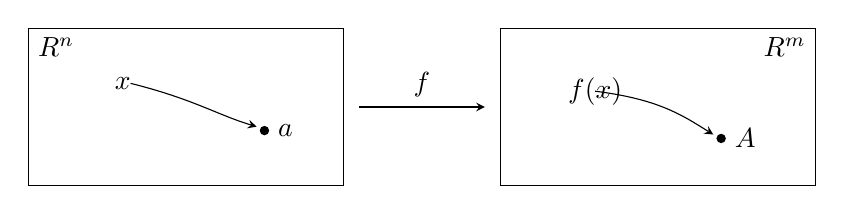
\begin{tikzpicture}[>=stealth]
  \draw (0,0) rectangle (4,2);
  \node[anchor=north west] at (0,2) {$\mathbb{R}^n$};
  \node at (1.2,1.3) {$x$};
  \draw[->] (1.3,1.3) .. controls (2.1,1.1) and (2.4,0.9) .. (2.9,0.75);
  \node[circle, fill, inner sep=1.2pt] at (3.0,0.7) {};
  \node[anchor=west] at (3.05,0.7) {$a$};

  \draw (6,0) rectangle (10,2);
  \node[anchor=north east] at (10,2) {$\mathbb{R}^m$};
  \node at (7.2,1.2) {$f(x)$};
  \draw[->] (7.2,1.2) .. controls (8.0,1.1) and (8.3,0.9) .. (8.7,0.65);
  \node[circle, fill, inner sep=1.2pt] at (8.8,0.6) {};
  \node[anchor=west] at (8.85,0.6) {$A$};

  \draw[->] (4.2,1) -- (5.8,1) node[midway, above] {$f$};
\end{tikzpicture}
\end{center}
\end{AnswerBox}\vspace{2mm}
\DefItem{Kontinuitet av en funktion från $\mathbb{R}^n$ till $\mathbb{R}^m$}{föreläsning 4 (se även sid 89 för $n=2,m=1$)}

\subsection{Derivator, differentierbarhet och linjär algebra för avbildningar}
\DefItem{Partiell derivata för en funktion från $\mathbb{R}^2$ till $\mathbb{R}$}{sid 94, eller föreläsning 5}
\DefItem{Differentierbarhet för en funktion från $\mathbb{R}^2$ till $\mathbb{R}$}{föreläsning 6 (obs! bokens definition på sid 103 skiljer sig något)}
\DefItem{Funktionalmatris/Jacobimatris för en funktion från $\mathbb{R}^n$ till $\mathbb{R}^m$}{sid 190, eller föreläsning 6}
\DefItem{Linjärisering av en funktion från $\mathbb{R}^n$ till $\mathbb{R}^m$}{föreläsning 6 (obs! boken använder begreppet annorlunda; båda tolkningar rätt)}

\subsection{Gradient och riktningsderivata}
\DefItem{Gradienten av en funktion från $\mathbb{R}^n$ till $\mathbb{R}$}{föreläsning 8 (se sid 99 för $n=2$)}
\DefItem{Riktningsderivata av en funktion från $\mathbb{R}^n$ till $\mathbb{R}$}{föreläsning 8 (se sid 101 för $n=2$)}

\subsection{Optimering}
\DefItem{Lokalt maximum/minimum för en funktion från $\mathbb{R}^n$ till $\mathbb{R}$}{föreläsning 11 (se sid 150 för $n=2$)}
\DefItem{Lokal extrempunkt och lokalt extremvärde för en funktion från $\mathbb{R}^n$ till $\mathbb{R}$}{föreläsning 11 (se sid 151 för $n=2$)}
\DefItem{Stationär punkt och sadelpunkt till en funktion från $\mathbb{R}^n$ till $\mathbb{R}$}{föreläsning 11 (se sid 152 för $n=2$)}
\DefItem{Hessematris/Hessianen för en funktion från $\mathbb{R}^n$ till $\mathbb{R}$}{föreläsning 11}
\DefItem{Globalt maximum/minimum för en funktion från $\mathbb{R}^n$ till $\mathbb{R}$}{föreläsning 12 (se även sid 162 för begreppet global extrempunkt)}

\subsection{Integraler och koordinatbyten}
\DefItem{Riemannsumma för en funktion från $\mathbb{R}^2$ till $\mathbb{R}$}{sid 253, eller PowerPoint på föreläsning 13}
\DefItem{Sambandet mellan kartesiska och polära koordinater samt areaelement}{sid 46, 199, eller föreläsning 2 \& 14}
\DefItem{Sambandet mellan kartesiska och sfäriska/rymdpolära koordinater samt volymelement}{sid 52, 200, eller föreläsning 2 \& 16}
\DefItem{Sambandet mellan kartesiska och cylindriska koordinater samt volymelement}{föreläsning 2 \& 16 (se även sid 49)}
\DefItem{Medelvärde av en reellvärd funktion av två/tre variabler på ett område}{föreläsning 17}

\subsection{Kurvor och kurvintegraler}
\DefItem{Parametrisering av en kurva}{sid 66 \& 67 (se även föreläsning 8 \& 18)}
\DefItem{Hastighet, fart och accelleration för en parametriserad rörelse}{föreläsning 18 (se även sid 184--185)}
\DefItem{Enkel, sluten, sammansatt och orienterad kurva}{sid 211 \& 212, eller föreläsning 18}
\DefItem{Bågelementet för en parametriserad kurva}{sid 275, eller föreläsning 18}
\DefItem{Integralen av funktion över kurva (kurvintegral) och längden av en kurva}{sid 274--276, 278, eller föreläsning 18}

\subsection{Vektorfält och potential}
\DefItem{Fältlinje till vektorfält}{föreläsning 19}
\DefItem{Tangentkurvintegral (kurvintegral av vektorfält)}{sid 285, 328, eller föreläsning 19}
\DefItem{Konservativt vektorfält (potentialfält) och potential}{sid 303, 328, 329, eller föreläsning 21}
\DefItem{Enkelt sammanhängande mängd/område}{sid 312, 343, eller föreläsning 21}
\DefItem{Ekvipotentialkurvor till plana konservativa vektorfält}{föreläsning 21}
\DefItem{Ekvipotentialytor till konservativa vektorfält i rummet}{föreläsning 21}

\subsection{Ytor, ytintegraler och differentialoperatorer}
\DefItem{Parametrisering av en yta}{sid 69, eller föreläsning 22}
\DefItem{Areaelementet för en parametriserad yta}{sid 279, eller föreläsning 22}
\DefItem{Integralen av funktion över yta (ytintegral) och arean av en yta}{sid 279, 281, eller föreläsning 22}
\DefItem{Orientering av yta}{sid 215, eller föreläsning 23}
\DefItem{Normalytelement för en yta}{föreläsning 23}
\DefItem{Normalytintegral/Flödesintegral (ytintegral av vektorfält)}{sid 332, eller föreläsning 23}
\DefItem{Divergensen och rotationen av vektorfält}{sid 324, 322 (plan); sid 348, 336 (rum), eller föreläsning 24}
\DefItem{Divergensfritt/Källfritt vektorfält}{sid 325, 354, eller föreläsning 24}
\DefItem{Rotationsfritt/Virvelfritt vektorfält}{sid 323, 342, eller föreläsning 24}

% ============================================================
\section{Formulera (utan bevis)}

\subsection{Derivator, kedjeregel och (im)plicita satser}
\ThmItem{Kedjeregeln för sammansättningar $\mathbb{R}\to\mathbb{R}^2\to\mathbb{R}$}{Sats 4.4, sid 110, eller föreläsning 7}
\ThmItem{Kedjeregeln för sammansättningar $\mathbb{R}^p\to\mathbb{R}^n\to\mathbb{R}^m$}{föreläsning 7}
\ThmItem{Gradienten är vinkelrät mot nivåytorna (för $f:\mathbb{R}^3\to\mathbb{R}$)}{Sats 4.9, sid 119, se även föreläsning 8}
\ThmItem{Inversa funktionssatsen (för $\mathbb{R}^2\to\mathbb{R}^2$)}{Sats 6.1, sid 202, se även föreläsning 9}
\ThmItem{Implicita funktionssatsen (för $\mathbb{R}^2\to\mathbb{R}$)}{Sats 6.2, sid 204, se även föreläsning 9}

\subsection{Taylor och optimering}
\ThmItem{Taylors formel t.o.m. andra ordningen (för $\mathbb{R}^2\to\mathbb{R}$)}{Sats 5.1, sid 147 (restterm: lättsam hantering duger)}
\ThmItem{Villkor för lokala extrempunkter}{Sats 5.3, sid 157, eller föreläsning 11}
\ThmItem{Villkor för extrempunkt under bivillkor}{Sats 5.4 (sid 171) och Sats 5.5 (sid 176), se även föreläsning 12}

\subsection{Integraler}
\ThmItem{Kontinuerliga funktioner är integrerbara}{Sats 7.2, sid 222, eller föreläsning 13}
\ThmItem{Upprepad integration i dubbelintegraler}{Sats 7.3 (sid 224) och Sats 7.7 (sid 231), se även föreläsning 13}
\ThmItem{Variabelbyte i dubbelintegraler}{Sats 7.8, sid 238, eller föreläsning 14}
\ThmItem{Variabelbyte i trippelintegraler}{analogt med dubbelintegraler (se även sid 257 eller föreläsning 16)}
\ThmItem{Medelvärdessatsen}{Sats 7.5, sid 228, eller föreläsning 17}

\subsection{Integralsatser och konservativa fält}
\ThmItem{Greens formel}{Sats 9.1, sid 291, eller föreläsning 20}
\ThmItem{Ekvivalenta villkor för konservativa fält}{sid 313, eller föreläsning 21}
\ThmItem{Virvelfria fält är konservativa (plan + rum)}{Sats 9.9 (sid 323) och Sats 10.3 (sid 344)}
\ThmItem{Gauss divergenssats}{Sats 10.4, sid 349, eller föreläsning 24}
\ThmItem{Stokes sats}{Sats 10.1, sid 338, eller föreläsning 25}

% ============================================================
\section{Formulera och bevisa/motivera}
\textit{Obs! På tentan kan även delar av nedanstående bevis/motiveringar efterfrågas.}

\subsection{Gradient, riktningsderivata och nivåmängder}
\ProofItem{Sats: $f_v'(a)=\nabla f(a)\cdot v$}{föreläsning 8 (se även Sats 4.6, sid 114, för två variabler)}
\ProofItem{Sats: riktningsderivatan är maximal i gradientens riktning}{föreläsning 8 (se även Sats 4.7, sid 116, för två variabler)}
\ProofItem{Sats: gradienten är vinkelrät till nivåkurvorna (för $\mathbb{R}^2\to\mathbb{R}$)}{Sats 4.8, sid 118, eller föreläsning 8}

\subsection{Kurvor och arbete}
\ProofItem{Formel för kurvlängd}{sid 274--275, eller föreläsning 18}
\ProofItem{Tangentkurvintegral som arbete (kurvintegral av vektorfält)}{sid 284--285, 328, eller föreläsning 19}
\ProofItem{Sats om tangentkurvintegraler över konservativa vektorfält}{Sats 9.3, sid 304, 329, eller föreläsning 21}

\subsection{Ytor och flöde}
\ProofItem{Formel för area av yta}{sid 279, eller föreläsning 22}
\ProofItem{Normalytintegral som flöde (ytintegral av vektorfält)}{sid 331--332, eller föreläsning 23}

\subsection{Greens och Gauss (bevisuppgifter)}
\ProofItem{Sats: varje konservativt vektorfält är virvelfritt}{Sats 10.2, sid 342, eller föreläsning 25}
\ProofItem{Bevisa Greens formel för områden som är både $y$-enkla och $x$-enkla}{bevis av formel 9.8, sid 300--301, och föreläsning 20}
\ProofItem{Bevisa Gauss sats för $F=(0,0,F_3)$ på $z$-enkla områden}{bevis av formel 10.15, sid 349--351, eller föreläsning 24}

\end{document}
